% Cover letter using letter.sty
\documentclass{letter} % Uses 10pt
%Use \documentstyle[newcent]{letter} for New Century Schoolbook postscript font
% the following commands control the margins:
\topmargin=-1in    % Make letterhead start about 1 inch from top of page 
\textheight=8in  % text height can be bigger for a longer letter
\oddsidemargin=0pt % leftmargin is 1 inch
\textwidth=6.5in   % textwidth of 6.5in leaves 1 inch for right margin
\usepackage[american]{babel}

\usepackage [autostyle, english = american]{csquotes}
\usepackage[version=3]{mhchem} 
\usepackage[hidelinks]{hyperref}
\usepackage{color}
\usepackage[ampersand]{easylist}
\usepackage{graphicx}
\usepackage{float}
\usepackage{caption}
\usepackage{amsmath}


\newfloat{figure}{htbp}{figs}

% \newcommand{\colornote}[1]{\textcolor{red}{ COMMENT\large\footnote{\textcolor{red}{#1}}}}
\newcommand{\colornote}[1]{\textcolor{red}{#1}}
\newcommand{\sci}[2]{ #1 \cdot 10^{#2}\ }
\newcommand{\pp}[1]{\left( #1\right)}


\begin{document}

\signature{Andrew S. Voyles}           % name for signature 
\longindentation=0pt                       % needed to get closing flush left
\let\raggedleft\raggedright                % needed to get date flush left
\date{13 May, 2020}

 
 
\begin{letter}{Dr. Jose Benlliure \\
Editor \\
European Physical Journal A}


\begin{flushleft}
{\large\bf Andrew S. Voyles, Ph.D.}
\end{flushleft}
\medskip\hrule height 1pt
\begin{flushright}
% \hfill The University of California, Berkeley \\
\hfill Lawrence Berkeley National Laboratory \\
\hfill Building 088-163D  |  M/S 88R0192, Berkeley, CA  94720-1730 \\
% \hfill (presently) +47 486 43 444 \\ 
\hfill  +1 (850) 281-0217 (mobile) or +1 (510) 486-7310 (office) 
\end{flushright} 
\vfill % forces letterhead to top of page

 
\opening{Dear Dr. Benlliure,} 

  \renewcommand*{\thefootnote}{\alph{footnote}}

  \noindent I am writing to submit my point-by-point responses to the issues raised by the reviewers for my submitted manuscript entitled \enquote{\emph{Proton-induced reactions on Fe, Cu, \& Ti from threshold to 55 MeV}},  for publication in European Physical Journal A.  Please find my responses detailed in \colornote{red text.}
  
  \noindent Along with my co-authors, I wanted to take the opportunity to personally thank you for your continued assistance in helping along the process of our submitted manuscript, and for finding such thorough and conscientious referees for reviewing it.  We would especially like to thank the referees for their thorough reading and critique, which has made it a better paper. Their comments were very constructive and pointed out some valuable improvements.
  
  
  \colornote{Lee - should we make any comments about the hostility and unhelpful/incorrect comment from Reviewer 1 here?}
  
  Please find the feedback following here, and our revised manuscript attached. 
  
  Sincerely yours,\\ \\ \\ \\ Andrew S. Voyles
 
% \closing{Sincerely yours,} 

  \vfill
  
 \pagebreak
 
 
 
 Referee \#1:
 
Authors have measured cross sections of the natFe(p,x), natCu(p,x) and natTi(p,x) reactions and done
model calculations using several codes with default parameters. No meaning of model calculations using
default parameter, author should adjust input parameter to fit experimental data.
It seems the paper related to measure cross sections for production of medical isotopes via proton
induced reactions on natFe, which play role to optimize production route; impurities, optimum energy
window, yield, etc. In this paper the above objects are not clearly presented. I would like to suggest to
calculate integral yields and discuss in details.
No meaning of the natCu(p,x) and natTi(p,x) reactions cross section measurements except monitor
reactions. Excitation functions of the monitor reactions induced on Cu and Ti should be determined and
compared with the IAEA recommended curve, which confirms experimental techniques and beam
parameters. Therefore, other reactions from Cu and Ti monitor should be omitted from the paper.

 \colornote{We thank the reviewer for their thoughtful comments....\\\\ ???????}


%   \colornote{We would first like thank the reviewer for their  detailed summary and suggestions of the manuscript. It is clear that they read the manuscript thoroughly, and the feedback they have provided here has been vital for the improvement of the paper as a whole.}


Few more comments:

1. P-2, line-15, ‘...........our measured data to probe the role of angular momentum...’.It should
clear and details in discussion.

2. Sample size 2.5 cm x2.5 cm is too large. What is the benefit of such sample size?

3. The notifications ’25 MeV stack’ and ’55 MeV stack’ are not correct.

4. Fig.1 is not special. Setup of 88-inch cyclotron is well characterized. The Fig. 1 should be
omitted.

5. In Fig.2, peak should be identified by energy and nuclide, not by symbol.

6. In Fig.3, why the trend of one stack is different from other.

7. EoB should be replaced by EOB.

8. What is the meaning of value in bracket in Tables.

\colornote{Uncertainties are listed in the least significant digit (NDS Style), that is, 131.0(85)\,mb  means 131.0 $\pm$ 8.5\,mb. Clarification to this effect has been added to the caption of all tables.}

9. P-8, line 44, ‘The natFe, natCu and natTi(p,x)......’ is not proper writing.

10. Both the numerical values for all investigated reactions should be given in Table and discussed in
details. But author did not discuss details for the reactions in Appendix.

\colornote{We thank your for this important feedback. We have since greatly expanded the language to include discussion of a dozen additional reaction channels of note, as well as their comparison with model calculations and prior data. As the large volume of cross section data we reported here  impacts  many applications,  we have added this new discussion to help show the importance of these results.}

Furthermore, the English and Writing as well as presentation is very poor. I can not recommend for
publication in the present form. It should be revised.





 
 
\pagebreak


 Referee \#2:



The paper \enquote{Proton-induced reactions on Fe, Cu, \& Ti from threshold to 55 MeV} describes three (six) comprehensive measurement campaigns obtaining data for the production of radioactive nuclides produced by the interaction of protons with natural iron, copper and titanium. The purpose is the determination of accurate excitation curves in support of investigations into alternative or optimized routes for the production of medical radionuclides. The authors use state of the art methods that are described in some detail in this paper and in some further detail in earlier papers involving some of the authors. Two stacks were irradiated for each material at two different energies 55 MeV and 25 MeV. Proton energy is further varied by energy loss straggling in the stack allowing up to 14 different energies from 4 to 53 MeV. The issues with this method concern the proper estimates of average proton energy per foil and the actual flux spectrum. The method is corrected/calibrated using monitor foils with well-determined cross sections but different energy dependence. The spread in results for these monitor foils has to be minimized by the estimates of proton energy and proton fluence spectra. Two methods are used. The first involves the use of FLUKA, a well-known simulation code with a long record of use in a variety of problems. The other method is not clearly described. The uncertain foil thicknesses (Al degraders, and kapton for 25 MeV) were adjusted to minimize the variation in fluence estimates from the one but last stack of monitor foils. The success of the method is demonstrated in Figure 3.
Provided the comments below are clarified, a large number of important new results are obtained. For reactions studied earlier, the accuracy is better than previous single measurements and the agreement with earlier results is good. There are a large number of reaction channels with first data (9 excitation curves, 7 for cross sections and 2 for branching ratios). By itself, these excellent new data obtained by careful experimental methods warrant accepting this publication, after taking care of the modifications suggested below. The paper further offers a clear warning against unchecked use of model calculations, even if performed with the latest developments in nuclear modelling codes. For work requiring even modest accuracy (say 20\%), these codes cannot be used to satisfaction. This warning may be more clearly highlighted in the conclusions of this paper.


\colornote{We would first like thank the reviewer for their  detailed summary and suggestions of the manuscript. It is clear that they read the manuscript thoroughly, and the feedback they have provided here has been vital for the improvement of the paper as a whole.}

Improve the description of the fitting method for minimizing the variance in the experimental fluence. The method is not clear now. Does this use AZ stopping powers and some semi-analytical approach? Expressions used?

\colornote{We thank you for raising this point, and apologize for this being unclear - we attempted to avoid duplication of much of the extensive discussion for this technique, as detailed in our previous work. We have now expanded upon this discussion in section 2.4, to make our methods more clear.  \\\\In short, FLUKA transport simulations were performed multiple times, globally perturbing the effective areal density (as a correction for the FLUKA stopping power model) of the aluminum degraders. Since each energy compartment, containing a Ti , Fe, and  Cu foil, within our stack has 4 independent monitor reactions, the perturbation in degrader density seeks to find which iteration minimizes the standard deviation of these 4 measurements, as the energy spectra from this iteration will best reproduce the IAEA-recommended monitor standard data. Since the thresholds and peaks of these different monitor reactions occur at different energies, a larger variance will be seen as the energy assignments are further away from those that reproduce the IAEA monitor data.  This is shown in a simple example in the attached figure.  So, no expressions are used here - simply finding the iteration which minimizes the standard deviation of the monitor reaction fluences.}

\begin{figure}
 \centering
 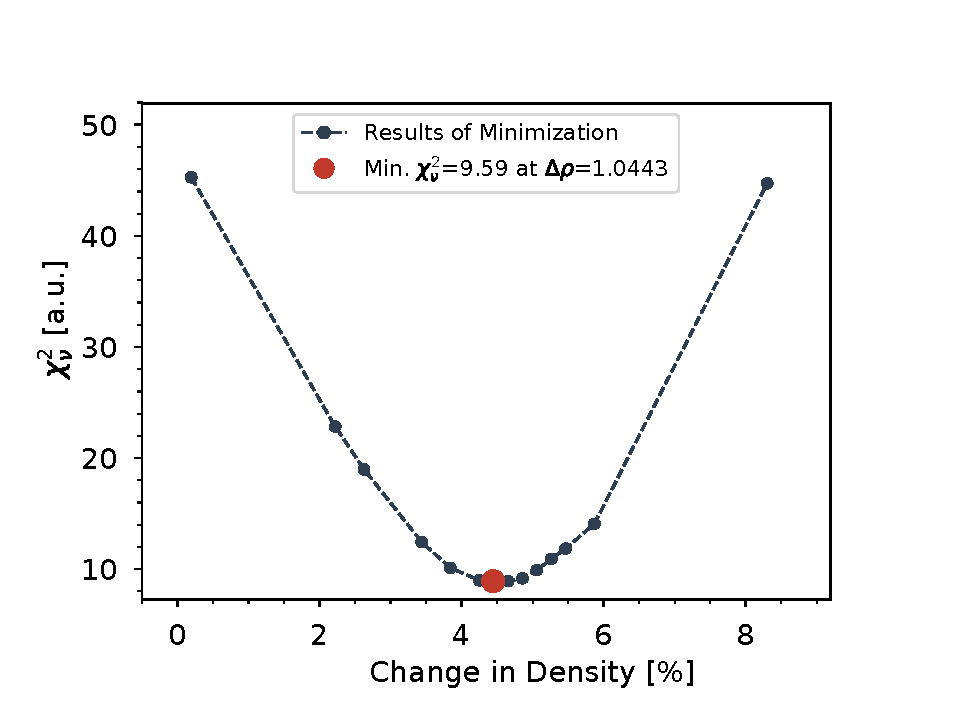
\includegraphics[width=0.7\textwidth]{./minimize_fluka_55.pdf}
 % sample_gspec.pdf: 489x257 pixel, 72dpi, 17.25x9.07 cm, bb=0 0 489 257
%  \caption{A gamma spectrum  from an activated Fe foil at approximately 55\,MeV (the maximum incident proton energy), collected 25 minutes after end-of-bombardment. Several observed reaction products are visible in this spectrum, and  the \ce{^{51}Cr} and \ce{^{52m}Mn} decay lines, which form two of the   primary reaction channels of interest, are  clearly isolated from surrounding peaks. }
%  \label{fig:gspec_femn}
\end{figure}

\colornote{Additionally, I removed the language in this section comparing the minimization results between AZ calculations and FLUKA, as well as Figure 4, which attempted to visually convey this, but I fear caused more confusion than it helped.  Most of the information needed is found in Figure 3B already, so this also helps avoid unnecessary duplication. Since we do not use the linear fit, AZ fluences estimates, or the FLUKA fluence model for any of our actual analysis,  having these in here might have partly led to the confusion.  Of all of this, only the FLUKA energy spectra (which lead to fluences when normalizing to IAEA monitor data) is actually used in our analysis, so I cut the rest to avoid any confusion in the final manuscript.  I hope that helps clarify things for you!}


The 55 MeV and 25 MeV irradiations have overlap: some energies are covered by both irradiations. This can be used to check the consistency of the methods used. However, the results do not clarify which results were obtained with which irradiation so that the reader cannot assert this consistency. Please, clearly specify which data were obtained from each of the two irradiations and show how consistent these are. A new plot or table may be necessary.

\colornote{We thank you for this very thoughtful suggestion. Running two overlapping stacks to build confidence through consistency was our goal for this, but the assignment of each foil to a stack is not clear, as you point out.  Tables 1--4, containing all of the measured cross section and ratio data, have all had a new row added, clearly designating the foil corresponding to each proton energy.}

The discussion speaks about the natural iron results in some detail, but almost nothing is said about the irradiations of natural copper and titanium. Please expand the discussion to obtain a fair description of all results.

I strongly suggest creating three figures in the main text, one for each of the irradiate materials (i.e. take these out of the annex). They should support the discussion about the results. In principle, a discussion should follow the pattern: short statements about the comparison to earlier work by channel, short statements about the agreement with models by channel; overall agreement to earlier data and to particular models. Of course, a grouped approach can be taken (several channels of a given nature). Separate messages about the data and their agreement with model estimates from the potential use of the results. Usefulness of the results should be either in the introduction or in an outlook at the end. There is also where implications should be highlighted (outlook at the end of the paper).



\colornote{We thank your for this important feedback. We have since greatly expanded the language to include discussion of a dozen additional reaction channels of note, as well as their comparison with model calculations and prior data. Your point that this new data warrants publication was very well-received, and we have added this new discussion to help show the importance of these results.}


Highlight clearly in the conclusions that model estimates are inadequate for even modest accuracy targets (like 20\%).

\colornote{We thank your for making this important point particularly clear. This point is a vital takeaway from this work, which was not made explicit enough, but has now been more directly addressed in the conclusions.}

If each activation foil is covered on both sides with kapton adhesive then this could be more clearly explained by either a drawing or the explicit mention of this in the tables describing the stacks.Please make this very explicit and mention clearly the best estimates for composition and thickness of these foils.

\colornote{We thank your for this point.  The language in section 2.1 has been updated to reflect this, and a short statement to this effect has been added to the caption of Table 6.}

 

 
% \encl{}  				% Enclosures

\end{letter}
 

\end{document}